\section{Heavy-light dekompozicija}

\subsection{Definicija}

Neka je $T = (V,E)$ stablo sa korenom $r \in V$. Za svaki \v cvor $x$ koji ima bar jedno dete defini\v semo $h_x$ na slede\' ci na\v cin. Neka su $y_1, \ldots, y_k$ sva deca \v cvora $x$. Tada je $h_x$ dete \v cije je podstablo najve\' ce odnosno koje ima najve\' ci broj potomaka. Ukoliko ovaj izbor nije jedinstven, uzima se bilo koje dete.

Posmatrajmo usmeren graf $H$ \v ciji je skup \v cvorova $V$ a skup grana je $\{(x, h_x) | x \text{ ima decu}\}$. Doka\v zimo da je on jednak uniji puteva. Svaki \v cvor ima ulazni stepen najvi\v se $1$, zato \v sto je jedina grana koja mo\v ze da ide ka njemu ona koja polazi iz njegovog roditelja. Tako\dj e, jasno je da svaki \v cvor po definiciji ima izlazni stepen najvi\v se $1$. Odavde zaklju\v cujemo da se graf mo\v ze razbiti na komponente, gde je svaka ili put ili ciklus. Ovaj graf ne sadr\v zi cikluse jer se du\v z svake \v setnje u grafu dubina \v cvora u stablu $T$ pove\' cava. Ovime smo pokazali da je $H$ razbijanje na puteve. Ovo razbijanje upravo zovemo \textit{Heavy-light dekompozicijom} stabla. U stablu $T$ grane $(x, h_x)$ nazivamo te\v skim, dok sve ostale grane nazivamo lakim granama -- odatle poti\v ce i naziv \textit{Heavy-light dekompozicija}.

\begin{figure}[H]
    \centering
    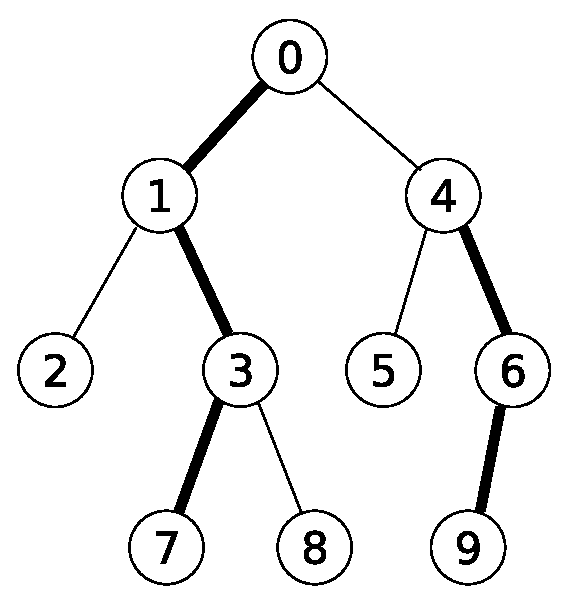
\includegraphics[width=80mm]{../img/hld.eps}
    \caption*{\textit{Primer heavy-light dekompozicije, koren je \v cvor 0. Te\v ske grane su podebljane.}}
\end{figure}

Ovo razbijanje je od zna\v caja jer zadovoljava slede\' cu veoma va\v znu osobinu.

\begin{thm}
\label{teoremalakegrane}
Neka je $T$ stablo sa $n$ \v cvorova sa korenom u $r$ a $H$ njegova Heavy-light dekompozicija. Neka je $x$ proizvoljan \v cvor. Posmatrajmo skup puteva u $H$ kojima pripadaju \v cvorovi na putu od $x$ do $r$. Tada ovaj skup sadr\v zi ne vi\v se od $\log_2(n) + 1$ elemenata.
\end{thm}

\textit{Dokaz.} Posmatrajmo put od $x$ do $r$ u $T$, i neka je taj put $p_1, p_2, \ldots, p_k$, gde je $k = d(x)+1$. Posmatrajmo dva uzastopna \v cvora sa tog puta, recimo $u,v$. Ako je grana $\{u,v\}$ laka, tada je $s(v) \geq 2s(u)$. Zaista, po\v sto je grana laka, $v$ ima jo\v s jedno dete $w$ razli\v cito od $u$ \v cija je veli\v cina podstabla $s(w)$ barem $s(v)$. Po\v sto je $s(v) \geq s(u) + s(w)$, direktno dobijamo tra\v zenu nejednakost. Ako grana nije laka, onda trivijalno va\v zi $s(v) \geq s(u)$. Jasno je da je broj razli\v citih puteva koji sadr\v ze \v cvorove na putu od $x$ do $r$ u $T$ za jedan ve\' ci od broja lakih grana na tom putu, jer svakim prelaskom lake grane dodajemo jedan novi put u $H$, dok prelaskom te\v ske grane ostajemo na istom putu u $H$. Dakle, neka je broj lakih grana $l$. Dokaza\' cemo da je $l \leq \log_2(n)$. Posmatrajmo niz brojeva $s(p_1), s(p_2), \ldots, s(p_k)$. Po\v sto je niz neopadaju\' c, $s(p_1) \geq 1$, a svaka laka grana zna\v ci da je slede\' ci broj bar duplo ve\' ci od prethodnog, imamo da je $n = s(r) = s(p_k) \geq 2^l$, odakle direktno dobijamo tra\v zenu nejednakost za $l$. Po\v sto je broj razli\v citih puteva $l+1$ ovime kompletiramo dokaz. \hfill $\square$.

\subsection{Algoritam za konstrukciju}

Za skladi\v svenje grana stabla koristi\' cemo listu susedstva. Konkretno, \v cvorove ozna\v cavamo brojevima od $0$ do $n-1$ i pamtimo niz nizova $e$, gde je $e[x]$ niz svih suseda \v cvora $x$. 
Koristimo \v sest pomo\' cnih nizova, svaki du\v zine $n$. To su:

\begin{itemize}
\item $p$ -- roditelj \v cvora. Slu\v zi nam da mo\v zemo da razlikujemo roditelja od dece nekog \v cvora, jer rekurziju radimo samo ka deci.
\item $h$ -- ukoliko $x$ ima dece, $h[x]$ je njegovo dete ka kojem ide te\v ska grana. U suprotnom $h[x] = -1$.
\item $d$ -- dubina \v cvora $x$ je $d[x]$. Za koren je dubina jednaka nuli.
\item $r$ -- koren, odnosno prvi \v cvor puta u $H$ kojem pripada \v cvor $x$ je $r[x]$.
\item $c$ -- konkatenacija svih puteva u $H$.
\item $pos$ -- inverz niza $c$, odnosno niz koji zadovoljava $pos[c[i]] = i$.
\end{itemize}

Algoritam se realizuje u dve faze. U prvoj fazi se pretragom u dubinu izra\v cunava veli\v cina svakog podstabla i odre\dj uju se te\v ske grane, odnosno vrednosti u nizu $h$. Pored toga, izra\v cunavaju se vrednosti u nizovima $p$ i $d$.

\noindent
\begin{minipage}{\textwidth}
\begin{lstlisting}[language=C++, title={Implementacija prve faze algoritma:}, style=customcpp]
int dfs(int x) {
	int shx = -1, sx = 1;
	for (int y : e[x]) {
		if (y != p[x]) {
			p[y] = x;
			d[y] = d[x] + 1;
			int sy = dfs(y);
			sx += sy;
			if (sy > shx) {
				shx = sy;
				h[x] = y;
			}
		}
	}
	return sx;
}
\end{lstlisting}
\end{minipage}

U drugoj fazi, na osnovu izra\v cunatih vrednosti u nizu $h$ se formiraju putevi, za svaki \v cvor se pamti koren njegovog puta i tako\dj e se u niz $c$ dodaju \v cvorovi sa tog puta. \v Cvor $x$ je koren nekog puta u $H$ ukoliko je on koren celog stabla, ili ako je grana koja spaja njega i njegovog roditelja laka, \v sto va\v zi ukoliko je $h[p[x]] \not = x$.

\noindent
\begin{minipage}{\textwidth}
\begin{lstlisting}[language=C++, title={Implementacija druge faze algoritma:}, style=customcpp]
void finish() {
	int n = e.size(), k = 0;
	for (int i=0; i<n; i++) {
		if (i == root || h[p[i]] != i) {
			for (int j=i; j!=-1; j=h[j]) {
				r[j] = i;
				c[k] = j;
				pos[j] = k++;
			}
		}
	}
}
\end{lstlisting}
\end{minipage}

U drugoj fazi se unutra\v snja for-petlja izvr\v sava ta\v cno jednom za svaki \v cvor, pa je vremenska i memorijska slo\v zenost obe faze $O(n)$. 

\subsection{Primene}

\subsubsection{k-ti predak \v cvora}

Za \v cvor $x$ i broj $k \geq 0$, $k$-ti predak je \v cvor $p^k(x)$, ukoliko postoji, za \v sta je dovoljan i potreban uslov da je $k \leq d[x]$. Algoritam za nala\v zenje ovog pretka je jednostavan. Ukoliko znamo da je taj predak u istom putu u $H$ kao $x$, \v sto mo\v zemo proveriti upore\dj ivanjem dubina \v cvorova $x$ i $r[x]$, samo se vratimo za $k$ mesta unazad u tom putu. U suprotnom, pretragu nastavljamo od \v cvora $p[r[x]]$ i $k$ smanjujemo za razliku u dubini.

\noindent
\begin{minipage}{\textwidth}
\begin{lstlisting}[language=C++, title={Implementacija algoritma za nala\v zenje k-tog pretka:}, style=customcpp]
int kth_ancestor(int x, int k) {
	if (d[x] < k)
		return -1;
	while (k > 0) {
		if (k <= d[x] - d[r[x]]) {
			return c[pos[x]-k];
		} else {
			k -= d[x] - d[r[x]] + 1;
			x = p[r[x]];
		}
	}
	return x;
}
\end{lstlisting}
\end{minipage}

Slo\v zenost algoritma je linearna po broju iteracija, odnosno po broju obi\dj enih lakih grana. Na osnovu teoreme \ref{teoremalakegrane} imamo da je vremenska slo\v zenost $O(\log n)$.

\subsubsection{Najni\v zi zajedni\v cki predak}

Posmatrajmo dva \v cvora stabla $x$ i $y$. Skupovi njihovih predaka se seku u bar jednom elementu -- u korenu stabla. Od svih njihovih zajedni\v ckih predaka, posmatrajmo onaj koji ima najve\' cu dubinu. Njega zovemo najni\v zim ili najdubljim zajedni\v ckim pretkom, u oznaci $LCA(x, y)$ (od \textit{Lowest common ancestor}). Ovaj \v cvor je jedinstveno odre\dj en, jer na putu od bilo kog \v cvora do korena nijedna dva \v cvora nemaju istu dubinu. \v Stavi\v se, presek puteva od $x$ do korena i od $y$ do korena stabla je upravo put od $LCA(x, y)$ do korena. Za \v cvor $LCA(x,y)$ va\v zi i da je put od $x$ do $y$ jednak konkatenaciji puteva od $x$ do $LCA(x,y)$ a zatim od $LCA(x,y)$ do $y$.

U kontekstu Heavy-light dekompozicije, nala\v zenje najni\v zeg zajedni\v ckog pretka je korisno i zato \v sto nam omogu\' cava da opi\v semo put izme\dj u svaka dva \v cvora kao uniju malog broja delova puteva iz Heavy-light dekompozicije, o \v cemu govori slede\' ca teorema:

\begin{thm}
\label{dveajkule}
Neka je $T = (V,E)$ stablo, $H$ njegova Heavy-light dekompozicija, i \v cvorovi $x,y \in V$. Skup puteva u $H$ koji sadr\v ze \v cvorove na putu u $T$ od $x$ do $y$ sadr\v zi ne vi\v se od $2\log_2(n)+1$ elemenata.
\end{thm}

\textit{Dokaz.} Na osnovu teoreme \ref{teoremalakegrane} znamo da je put od $x$ do korena u $T$ sadr\v zan u ne vi\v se od $\log_2(n)+1$ puteva u $H$. Isto va\v zi i za put od $y$ do korena. Unija ova dva skupa puteva ima bar jedan element manje, jer je presek tih skupova put u $H$ koji sadr\v zi koren stabla, odnosno ima ne vi\v se od $2(\log_2(n)+1) - 1 = 2\log_2(n)+1$ elemenata. Kako je put od $x$ do $y$ u $T$ podskup unije puteva od $x$ do $r$ i od $y$ do $r$, va\v zi i da \' ce taj put da bude sadr\v zan u ne vi\v se od $2\log_2(n)+1$ puteva u $H$. \hfill $\square$

Opi\v simo sada algoritam za nala\v zenje $LCA$ za neka dva \v cvora. Ideja je da pribli\v zavamo te \v cvorove korenu stabla, vode\' ci ra\v cuna da ne presko\v cimo stvarnu vrednost $LCA$. Za to \' ce nam pomo\' ci slede\' ca tvr\dj enja:

\begin{thm}
Ako je $r[x] = r[y]$, tada je $LCA(x,y) = x$ ukoliko je $d[x] < d[y]$, ina\v ce je $LCA(x, y) = y$.
\end{thm}

\textit{Dokaz.} Po\v sto je $r[x] = r[y]$ ova dva \v cvora se nalaze na istom putu u $H$, pa je jedan od njih drugome predak. $LCA$ je \v cvor na manjoj dubini. \hfill $\square$

\begin{thm}
Ako je $r[x] \not = r[y]$ i $d[r[x]] \leq d[r[y]]$, tada je $LCA(x,y) = LCA(x, p[r[y]])$.
\end{thm}

\textit{Dokaz.} Ukoliko je $z$ proizvoljan predak \v cvora $y$, tada je $LCA(x,z)$ ili jednako $z$, ili jednako $LCA(x,y)$, a oba va\v ze samo kad je $z=LCA(x,y)$.  Pretpostavimo suprotno, $LCA(x,y) \not = LCA(x, p[r[y]])$.  Po\v sto je $p[r[y]]$ predak \v cvora $y$, imamo da je $LCA(x, p[r[y]]) = p[r[y]]$ predak \v cvora $x$ a samim tim i \v cvora $LCA(x,y)$. Put od $y$ do $p[r[y]]$ sadr\v zi $LCA(x,y)$, a po\v sto je $LCA(x,y) \not = p[r[y]]$ onda je $r[y]$ predak \v cvora $LCA(x,y)$. Posmatrajmo sada put u $H$ koji sadr\v zi $x$. Taj put ne mo\v ze da sadr\v zi $LCA(x,y)$ jer on pripada putu \v ciji je koren $r[y]$, a iz uslova teoreme imamo da je $r[x] \not = r[y]$. Po\v sto je $LCA(x,y)$ predak \v cvora $x$, put u $H$ koji sadr\v zi $x$ mora da se zaustavi pre $LCA(x,y)$, pa je $d[r[x]] > d[LCA(x,y)] \geq d[r[y]]$ \v sto je u kontradikciji sa uslovom teoreme. \hfill $\square$

Ovo nam omogu\' cava da u jednoj iteraciji ili zaklju\v cimo da je jedan od \v cvorova LCA, ili da pribli\v zimo jedan \v cvor korenu preska\v cu\' ci ta\v cno jednu laku granu.

\noindent
\begin{minipage}{\textwidth}
\begin{lstlisting}[language=C++, title={Implementacija algoritma za nala\v zenje LCA:}, style=customcpp]
int lca(int x, int y) {
	while (r[x] != r[y]) {
		if (d[r[x]] > d[r[y]])
			swap(x, y);
		y = p[r[y]];
	}
	return d[x] < d[y] ? x : y;
}
\end{lstlisting}
\end{minipage}

Slo\v zenost algoritma je linearna po broju iteracija, odnosno broju presko\v cenih lakih grana, \v sto po teoremi \ref{dveajkule} iznosi ne vi\v se od $2\log_2(n)+1$ tj. $O(\log n)$.

\subsubsection{Obrada puteva u stablu}

Heavy-light dekompozicija nam omogu\' cava da probleme kod kojih treba na neki na\v cin obraditi put u stablu svedemo na sli\v cnu obradu $O(\log n)$ segmenata u nizu. Jedna od osnovnih struktura za obradu segmenata jeste \textit{segmentno stablo}. Ukratko, za niz elemenata $a_0, \ldots, a_{n-1}$ iz monoida $(A,+)$ segmentno stablo omogu\' cava da se u logaritamskoj slo\v zenosti izra\v cuna zbir elemenata bilo kog podsegmenta $a_l + a_{l+1} + \ldots + a_r$, kao i da se vr\v se izmene, odnosno dodele vrednosti elementima niza $a$. Tako se ove iste operacije mogu podr\v zati na putevima u stablu u vremenskoj slo\v zenosti $O(\log^2n)$.

Kod monoida koji nisu komutativni treba voditi ra\v cuna o redosledu elemenata, odnosno, za put od $u$ do $v$, deo puta od $u$ do $LCA(u,v)$ ide ka korenu stabla, odnosno, suprotno od smera puteva u $H$, dok od $LCA(u,v)$ do $v$ ide u smeru puteva u $H$, pa je potrebno napraviti jo\v s jedno segmentno stablo koje \v cuva obrnute sume.

Segmentno stablo se inicijalizuje zadavanjem veli\v cine $n$. Ono mo\v ze zauzeti do $4$ puta vi\v se memorije od one potrebne da se skladi\v sti niz sa $n$ elemenata.

\noindent
\begin{minipage}{\textwidth}
\begin{lstlisting}[language=C++, title={Inicijalizacija segmentnog stabla:}, style=customcpp]
template<class T>
class segment_tree {
	vector<T> a;
	int maxn;
	
	segment_tree(int n) {
		maxn = 1;
		while (maxn < n)
			maxn <<= 1;
		a.resize(2*maxn);
	}

	// ...
};
\end{lstlisting}
\end{minipage}

Izmena elemenata ima jednostavu iterativnu implementaciju.

\noindent
\begin{minipage}{\textwidth}
\begin{lstlisting}[language=C++, title={Izmena elementa u segmentnom stablu:}, style=customcpp]
void update(int x, T y) {
	x += maxn;
	a[x] = y;
	while (x > 1) {
		x >>= 1;
		a[x] = a[2*x] + a[2*x+1];
	}
}
\end{lstlisting}
\end{minipage}

Upit za podsegment tako\dj e ima jednostavnu implementaciju, ali je dokaz vremenske slo\v zenosti komplikovaniji. Obe operacije imaju vremensku slo\v zenost $O(\log n)$.

\noindent
\begin{minipage}{\textwidth}
\begin{lstlisting}[language=C++, title={Upit za sumu podsegmenta u segmentnom stablu:}, style=customcpp]
T query(int l, int r, int x, int xl, int xr) {
	if (r < xl || xr < l)
		return T();
	if (l <= xl && xr <= r)
		return a[x];
	int xm = (xl+xr) >> 1;
	return
		query(l, r, 2*x, xl, xm) +
		query(l, r, 2*x+1, xm+1, xr);
}

T query(int l, int r) {
	return query(l, r, 1, 0, maxn-1);
}
\end{lstlisting}
\end{minipage}

Kona\v cno, modifikacijom algoritma za nala\v zenje LCA podr\v zavamo upite na putevima u stablu kao i izmene vrednosti u \v cvorovima. Slede\' ca implementacija podrazumeva da je monoid vrednosti komutativan.

\noindent
\begin{minipage}{\textwidth}
\begin{lstlisting}[language=C++, title={Operacije na putevima sa izmenama:}, style=customcpp]
segment_tree<T> tree;
//...

void update(int x, T y) {
	tree.update(pos[x], y);
}

T query(int x, int y) {
	T sum = T();
	while (r[x] != r[y]) {
		if (d[r[x]] > d[r[y]])
			swap(x, y);
		sum = sum + tree.query(pos[r[y]], pos[y]);
		y = p[r[y]];
	}
	if (d[x] > d[y])
		swap(x, y);
	return sum + tree.query(pos[x], pos[y]);
}
\end{lstlisting}
\end{minipage}

Ukoliko se operacije na putevima odnose na obi\dj ene grane a ne \v cvorove, mo\v zemo za svaku granu stabla $\{u, v\}$ dodati jedan novi \v cvor (nazovimo ga $w$) a zatim zameniti tu granu dvema granama $\{u, w\}, \{w, v\}$. U originalnim \v cvorovima stabla \v cuvamo neutrale za monoid vrednosti. Cela implementacija zajedno sa re\v senjem zadatka \href{https://spoj.com/problems/QTREE}{QTREE} mo\v ze se na\' ci u dodatku \ref{sirkod}.